\documentclass[10pt]{article}
\usepackage[margin=0.75in,columnsep=0.3in]{geometry}
\usepackage{amsmath,amssymb}
\usepackage{booktabs}
\usepackage{graphicx}
\usepackage{caption}
\usepackage{enumitem}
\usepackage[colorlinks=true,linkcolor=blue,urlcolor=blue,citecolor=blue]{hyperref}

\setlength{\parindent}{0pt}
\setlength{\parskip}{0.5em}

\title{\vspace{-2em}}
\date{}

\begin{document}

\twocolumn[{
\centering
{\LARGE\bfseries A Purged, Embargoed Walk-Forward Backtester}\par
\vspace{6pt}
{\large Quantifying Look-Ahead-Bias Sharpe Inflation and Correcting for
Multiple-Testing Bias on a Real 15-Stock Equity Universe}\par
\vspace{10pt}
{\itshape Code: \href{https://github.com/yassineerraji/ML-Backtester-with-Strict-Anti-Look-Ahead-Bias}{GitHub Repository}
\ \textbar\ \ App: \href{https://ml-backtester-with-strict-anti-look-ahead-bias.streamlit.app}{Live Demo}}\par
\vspace{10pt}
Yassine Erraji\par
September 2026\par
\vspace{10pt}
}

\noindent\textbf{Abstract} This report documents a machine-learning signal-to-backtest pipeline built to make one specific bias visible and then remove it: the inflation of a walk-forward backtest's Sharpe ratio caused by training on samples whose label window overlaps the following test period. Two walk-forward splitters sharing one interface --- a naive splitter with no purge or embargo, and a corrected splitter implementing both --- are run on identical data (15 large-cap US equities, 2015--2024, daily bars), identical rolling-window features, an identical LightGBM regressor refit fresh on every fold, and identical transaction costs; only the validation methodology differs. On a train window sized so purge removes a material 16.7\% of each fold's training data (30 trading days, 5-day forward-return horizon), the naive splitter reports a Sharpe ratio of 1.57 against the corrected splitter's 0.46 --- a gap of 1.11 attributable purely to validation methodology, not to any difference in data, model, or costs. Because the corrected splitter also spends 5 trading days per fold on an embargo buffer, it fits fewer folds into the same date range (54 vs. 60), a second, more subtle source of naive-vs-corrected divergence, documented explicitly rather than hidden. Testing five LightGBM hyperparameter configurations on the corrected splitter and applying the deflated Sharpe ratio of Bailey and L\'opez de Prado shows the best-observed Sharpe of 1.26 survives the multiple-testing correction (deflated Sharpe 0.92), evidence the result is not simply the best of five random draws. A caching defect discovered while preparing this report --- an off-by-one interaction with Yahoo Finance's exclusive end-date semantics that silently forced a full data re-download on every run --- is also documented, since it had been quietly undermining the exact cross-run reproducibility the project's methodology depends on.

\vspace{1em}
]

\section{Introduction}

Backtested trading strategies are notoriously easy to overstate: a walk-forward validation that ignores the fact that a label's outcome is only known some days after it is observed will silently train on information from inside the period it is about to be tested on, and the resulting Sharpe ratio will read higher than any live strategy could achieve. This project builds that failure mode on purpose, quantifies it in Sharpe-ratio terms on real market data, and then removes it. Rather than building a single ``correct'' backtester and asserting it is unbiased, it builds two backtesters that share every component except the validation split, so the size of the bias is a number produced by running code, not a claim. Every result below comes from \texttt{ml\_backtester.experiments}, runs against a local Yahoo Finance cache under a fixed, literal \texttt{Config()} default, and is reproducible from a clean checkout. Section 2 documents a data-caching defect found and fixed specifically because it was silently breaking that reproducibility guarantee.

\section{Methodology \& Conventions}

The universe is 15 large-cap US equities (\texttt{DEFAULT\_UNIVERSE} in \texttt{config.py}); data is daily OHLCV pulled via \texttt{yfinance} and cached locally as parquet. Features --- momentum, realized volatility, relative volume, and RSI --- are computed from trailing rolling windows only and normalized against their own trailing window, never the full series, so no feature can see the future. Labels are the forward return over a 5-trading-day horizon; every observation additionally carries $t_1$, the timestamp at which its label is actually resolved --- the timestamp the purge rule in Section 3 keys off, rather than a row count or date offset.

The model is a LightGBM regressor, refit from scratch on every fold's training data alone and predicting only that fold's test rows --- never fit on the full dataset. Two settings were required for the pipeline itself to be bit-reproducible across separate process runs, independent of any modeling choice: \texttt{deterministic=True} plus \texttt{force\_row\_wise=True}, since LightGBM's default multi-threaded histogram construction is not guaranteed reproducible run-to-run even with a fixed random seed.

Positions are sized by cross-sectionally $z$-scoring the model's predicted return within each date, then clipping to a risk cap, so sizing reflects relative conviction rather than raw prediction magnitude. Costs are a fixed spread-plus-slippage in basis points, applied to every position change.

\textbf{Data-caching defect.} While preparing this report, the same \texttt{Config()} run produced three different Sharpe ratios (0.50, 0.49, 0.46) across three separate process invocations of otherwise identical code. The cause was not model nondeterminism: the local parquet cache's staleness check compared the \emph{returned data's} maximum date against the requested \texttt{end\_date}, but \texttt{yfinance}'s \texttt{end} parameter is exclusive, so returned data never actually reaches the requested end date. That comparison was therefore always true, silently forcing a full re-download from Yahoo Finance on every single call --- and Yahoo's adjusted-close values are not bit-stable across separate pulls. The fix records the \emph{requested} date range in a small sidecar metadata file and checks staleness against that instead of against the ambiguous returned range. Every number in this report was generated after the fix, confirmed bit-identical across three fresh process runs; the qualitative conclusion (naive Sharpe exceeds corrected) held both before and after, but exact reproducibility --- the property this project's own methodology depends on --- did not, until the cache was fixed.

\section{Walk-Forward Validation: Purge and Embargo}

Two splitters share one constructor and one \texttt{split()} signature: \texttt{WalkForwardSplitter} (naive), which applies neither correction, and \texttt{PurgedEmbargoedSplitter}, which applies both. \textbf{Purge} drops any training row whose label window overlaps the following test block --- concretely, any row with $t_1 \geq \text{test\_start}$. \textbf{Embargo} then skips a fixed number of trading days after each test block before the next training block may begin, absorbing residual autocorrelation across the boundary.

\begin{table}[h]
\centering
\begin{tabular}{lrr}
\toprule
 & Naive & Corrected \\
\midrule
Folds (2015--2024) & 60 & 54 \\
Fold 0 train rows & 450 & 375 \\
Rows purged, fold 0 & --- & 75 (16.7\%) \\
Fold 1 train start & 2015-06-24 & 2015-07-01 \\
\bottomrule
\end{tabular}
\caption{Fold structure with a 30-day train window, 10-day test window, 5-day embargo, 5-day label horizon. 75 rows purged $=$ 15 tickers $\times$ 5-day horizon.}
\end{table}

The 30-day train window is deliberately short relative to a multi-year institutional retrain cadence: the purged fraction equals horizon days over train-window days, so this project's 3-year default from an earlier iteration (756 days) purged only 0.7\% of each fold --- too little to move the Sharpe ratio noticeably, and too little to make the point this project exists to make. Figure 1 shows the first six folds of each variant: red bands mark dates that would leak into training if left uncorrected, computed identically for both variants so the comparison is direct; only the corrected splitter actually excludes them (there is no red band missing from the naive row --- the naive splitter keeps exactly the dates the corrected splitter discards). Purple embargo bands appear only for the corrected variant, and their presence is why it fits into six fewer folds over the same ten-year window.

\begin{figure}[h]
\centering
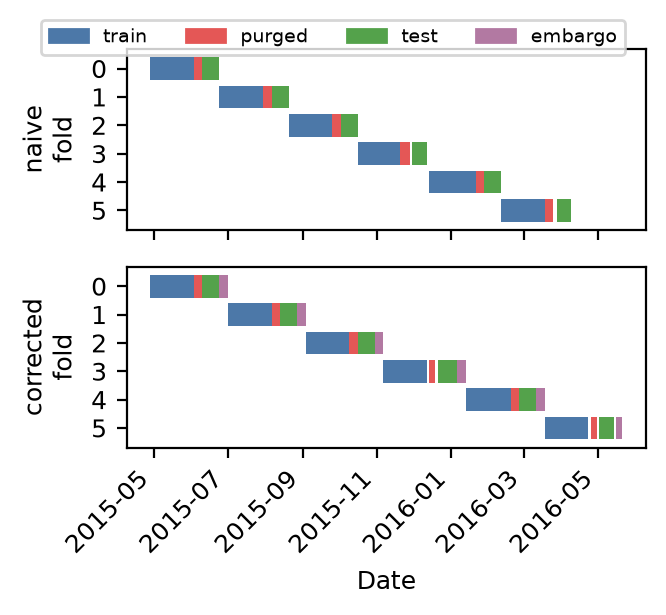
\includegraphics[width=\linewidth]{figures/fold_timeline.png}
\caption{First six folds, naive vs.\ corrected. Purged dates (red) are computed identically for both; only the corrected splitter removes them from training.}
\end{figure}

\section{Naive vs.\ Corrected Bias Comparison}

Table 2 reports out-of-sample metrics concatenated across every fold's test block, for the naive and corrected splitters run on identical data, features, model, and costs.

\begin{table}[h]
\centering
\begin{tabular}{lrr}
\toprule
Metric & Naive & Corrected \\
\midrule
Sharpe & 1.5717 & 0.4578 \\
Sortino & 2.4660 & 0.7281 \\
Max drawdown & $-$0.1498 & $-$0.2348 \\
Turnover & 0.0719 & 0.0783 \\
Hit ratio & 0.5383 & 0.5037 \\
\bottomrule
\end{tabular}
\caption{Naive vs.\ corrected walk-forward metrics, identical universe/model/costs.}
\end{table}

The Sharpe gap of 1.11 is not the only symptom. Hit ratio falls from 53.8\% to 50.4\% --- once corrected, the model's directional accuracy is close to indistinguishable from a coin flip. Maximum drawdown is \emph{worse}, not better, once corrected ($-$23.5\% vs.\ $-$15.0\%): the naive version does not merely overstate returns, it understates the real risk of the strategy it is validating. Figure 2 shows both cumulative equity curves; the corrected curve tracks the naive curve closely until roughly 2020, after which the two visibly diverge.

\begin{figure}[h]
\centering
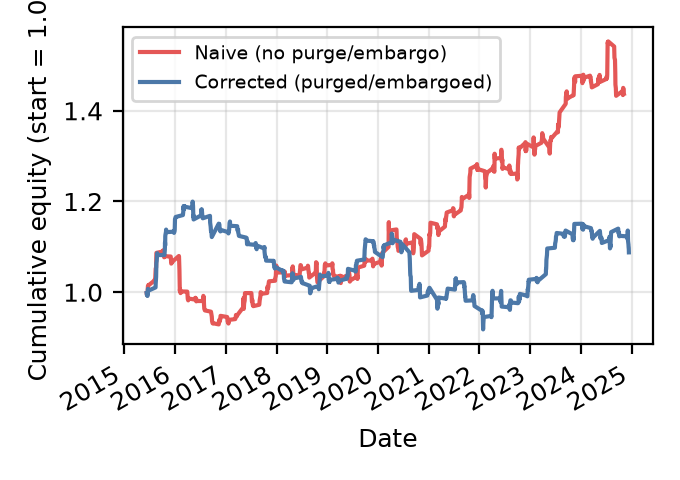
\includegraphics[width=\linewidth]{figures/equity_curves.png}
\caption{Cumulative out-of-sample equity, naive vs.\ corrected.}
\end{figure}

Part of this gap is methodological rather than purely a leakage artifact: because the corrected splitter spends time on the embargo gap, its 54 folds do not cover exactly the same calendar dates as the naive splitter's 60. The two runs are not evaluated on an identical set of test periods, so a small part of the divergence reflects that difference in coverage rather than the leak in isolation --- a limitation documented rather than hidden (Section 6).

\section{Deflated Sharpe Ratio: Correcting for Multiple-Testing Bias}

Reporting the best Sharpe found across several model configurations overstates skill: some configurations look good by chance alone, and that chance component grows with the number of configurations tried. Five LightGBM hyperparameter configurations were run on the corrected splitter, on identical data and costs, varying only \texttt{num\_leaves} and \texttt{max\_depth}.

\begin{table}[h]
\centering
\begin{tabular}{rrr}
\toprule
num\_leaves & max\_depth & Sharpe \\
\midrule
7 & 2 & 1.2613 \\
15 & 3 & 1.0048 \\
31 & 5 & 0.8405 \\
63 & 7 & 0.7469 \\
15 & 7 & 0.6523 \\
\bottomrule
\end{tabular}
\caption{Five-trial hyperparameter sweep, corrected splitter, annualized Sharpe.}
\end{table}

The best trial (\texttt{num\_leaves=7, max\_depth=2}) reaches an annualized Sharpe of 1.2613. Applying the deflated Sharpe ratio of Bailey and L\'opez de Prado --- which asks what Sharpe an average skill-less strategy would achieve by chance given five configurations were tried, and reports the probability the true Sharpe exceeds that benchmark --- gives a deflated Sharpe ratio of \textbf{0.9247}. A value this close to 1.0 indicates the best-observed result is unlikely to be a product of the search itself, in contrast to a value near 0.5, which would be indistinguishable from noise.

\begin{figure}[h]
\centering
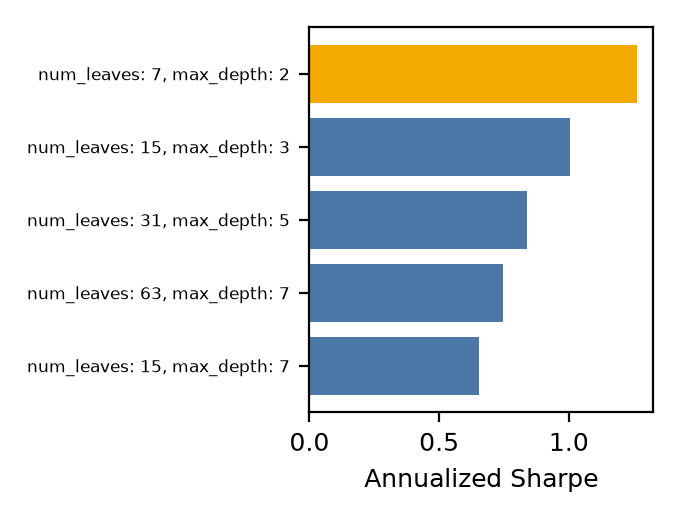
\includegraphics[width=\linewidth]{figures/sweep_bars.png}
\caption{Annualized Sharpe per trial; best trial highlighted.}
\end{figure}

This result should be read with one caveat: the deflation formula's assumption of independent trials is only approximate here, since all five configurations share both a model family and a dataset (Section 6).

\section{Limitations \& Future Work}

Five scope limits are worth naming rather than leaving implicit. The 15-name universe is not market-representative, and results --- including the sign and magnitude of the naive-vs-corrected gap --- are not claimed to generalize beyond this universe or period. The 30-day train window was chosen to make the leak visible, not because it is a realistic institutional retrain cadence; a multi-year window exhibits the same leak but purges too small a fraction to move the Sharpe ratio noticeably (Section 3). The naive and corrected runs do not cover identical calendar time, so part of the measured gap reflects differing test-period coverage rather than the leak in isolation (Section 4). The hyperparameter grid is small (five trials) and not fully independent, since every trial shares a model family and dataset --- the deflation formula's independence assumption is approximate. Finally, no financing or borrow costs are modeled, and every feature/label/cost choice draws from a single fixed configuration rather than a validated-elsewhere production setup.

\section{Conclusion}

Holding data, features, model, and costs fixed and varying only the walk-forward validation methodology produces a 1.11-point Sharpe gap, a materially worse realized drawdown once corrected, and a hit ratio that collapses toward chance --- three independent symptoms of the same underlying leak, not one number in isolation. A hyperparameter configuration that looks best among five trials survives the deflated Sharpe correction (0.92), evidence its outperformance is not simply the best of five random draws. Finally, a caching defect that had been silently reintroducing non-reproducibility into every reported number was found, fixed, and confirmed bit-identical across independent runs --- a reminder that a project built to catch one specific bias should not assume it is free of others.

\begin{thebibliography}{9}
\bibitem{lopezdeprado2018} M. L\'opez de Prado, \emph{Advances in Financial Machine Learning}. Wiley, 2018.
\bibitem{bailey2014deflated} D. Bailey and M. L\'opez de Prado, ``The Deflated Sharpe Ratio: Correcting for Selection Bias, Backtest Overfitting, and Non-Normality,'' \emph{Journal of Portfolio Management}, 40(5), 2014.
\bibitem{ke2017lightgbm} G. Ke et al., ``LightGBM: A Highly Efficient Gradient Boosting Decision Tree,'' \emph{Advances in Neural Information Processing Systems (NeurIPS)}, 2017.
\end{thebibliography}

\end{document}
